\documentclass[14pt]{extbook}
\usepackage{multicol, enumerate, enumitem, hyperref, color, soul, setspace, parskip, fancyhdr} %General Packages
\usepackage{amssymb, amsthm, amsmath, bbm, latexsym, units, mathtools} %Math Packages
\everymath{\displaystyle} %All math in Display Style
% Packages with additional options
\usepackage[headsep=0.5cm,headheight=12pt, left=1 in,right= 1 in,top= 1 in,bottom= 1 in]{geometry}
\usepackage[usenames,dvipsnames]{xcolor}
\usepackage{dashrule}  % Package to use the command below to create lines between items
\newcommand{\litem}[1]{\item#1\hspace*{-1cm}\rule{\textwidth}{0.4pt}}
\pagestyle{fancy}
\lhead{Makeup Progress Quiz 1}
\chead{}
\rhead{Version C}
\lfoot{6018-3080}
\cfoot{}
\rfoot{Spring 2021}
\begin{document}

\begin{enumerate}
\litem{
Write the equation of the line in the graph below in Standard form $Ax+By=C$. Then, choose the intervals that contain $A, B, \text{ and } C$.
\begin{center}
    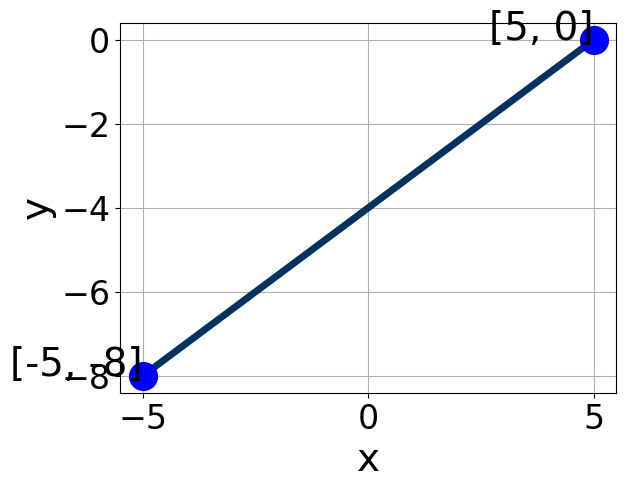
\includegraphics[width=0.5\textwidth]{../Figures/linearGraphToStandardCopyC.png}
\end{center}
\begin{enumerate}[label=\Alph*.]
\item \( A \in [-3.8, 0.2], \hspace{3mm} B \in [-1, 0], \text{ and } \hspace{3mm} C \in [3, 5] \)
\item \( A \in [0, 8], \hspace{3mm} B \in [-11, -4], \text{ and } \hspace{3mm} C \in [20, 21] \)
\item \( A \in [-4, -3], \hspace{3mm} B \in [5, 8], \text{ and } \hspace{3mm} C \in [-20, -19] \)
\item \( A \in [0, 8], \hspace{3mm} B \in [5, 8], \text{ and } \hspace{3mm} C \in [-20, -19] \)
\item \( A \in [-3.8, 0.2], \hspace{3mm} B \in [1, 4], \text{ and } \hspace{3mm} C \in [-6, -1] \)

\end{enumerate} }
\litem{
Solve the linear equation below. Then, choose the interval that contains the solution.\[ \frac{3x + 9}{2} - \frac{-7x + 7}{6} = \frac{5x + 3}{3} \]\begin{enumerate}[label=\Alph*.]
\item \( x \in [-7.3, -3.5] \)
\item \( x \in [-4.3, -0.6] \)
\item \( x \in [0.4, 2.9] \)
\item \( x \in [-1.5, -0.2] \)
\item \( \text{There are no real solutions.} \)

\end{enumerate} }
\litem{
Solve the equation below. Then, choose the interval that contains the solution.\[ -2(-6x + 11) = -3(-7x -4) \]\begin{enumerate}[label=\Alph*.]
\item \( x \in [-2.2, -0.5] \)
\item \( x \in [-0.1, 0.8] \)
\item \( x \in [-4.2, -3] \)
\item \( x \in [0.9, 2.1] \)
\item \( \text{There are no real solutions.} \)

\end{enumerate} }
\litem{
Find the equation of the line described below. Write the linear equation as $ y=mx+b $ and choose the intervals that contain $m$ and $b$.\[ \text{Parallel to } 5 x + 4 y = 3 \text{ and passing through the point } (3, 4). \]\begin{enumerate}[label=\Alph*.]
\item \( m \in [-1.4, -0.9] \hspace*{3mm} b \in [-8.88, -7.26] \)
\item \( m \in [0.6, 1.57] \hspace*{3mm} b \in [-0.57, 0.55] \)
\item \( m \in [-0.82, -0.39] \hspace*{3mm} b \in [7.47, 8.06] \)
\item \( m \in [-1.4, -0.9] \hspace*{3mm} b \in [0.62, 1.33] \)
\item \( m \in [-1.4, -0.9] \hspace*{3mm} b \in [7.47, 8.06] \)

\end{enumerate} }
\litem{
Write the equation of the line in the graph below in Standard form $Ax+By=C$. Then, choose the intervals that contain $A, B, \text{ and } C$.
\begin{center}
    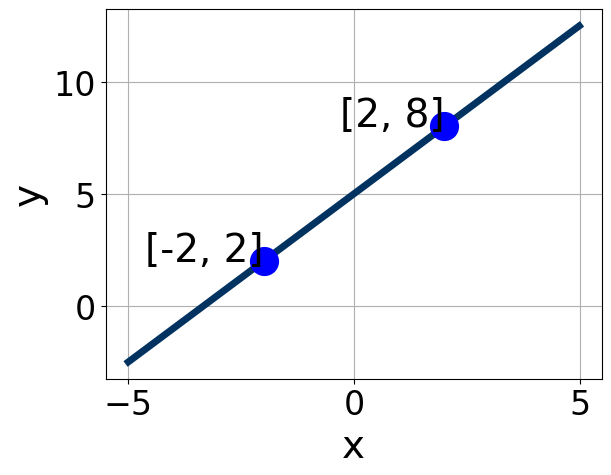
\includegraphics[width=0.5\textwidth]{../Figures/linearGraphToStandardC.png}
\end{center}
\begin{enumerate}[label=\Alph*.]
\item \( A \in [1.8, 5.8], \hspace{3mm} B \in [1.84, 2.16], \text{ and } \hspace{3mm} C \in [9.3, 10.3] \)
\item \( A \in [1.8, 5.8], \hspace{3mm} B \in [-2.42, -1.69], \text{ and } \hspace{3mm} C \in [-12.8, -7.6] \)
\item \( A \in [-3.3, -2.8], \hspace{3mm} B \in [1.84, 2.16], \text{ and } \hspace{3mm} C \in [9.3, 10.3] \)
\item \( A \in [-2.6, 0.7], \hspace{3mm} B \in [-1.1, 0.01], \text{ and } \hspace{3mm} C \in [-5.6, -1.5] \)
\item \( A \in [-2.6, 0.7], \hspace{3mm} B \in [0.99, 1.4], \text{ and } \hspace{3mm} C \in [3.2, 6.4] \)

\end{enumerate} }
\litem{
First, find the equation of the line containing the two points below. Then, write the equation as $ y=mx+b $ and choose the intervals that contain $m$ and $b$.\[ (2, -3) \text{ and } (5, 6) \]\begin{enumerate}[label=\Alph*.]
\item \( m \in [1, 7] \hspace*{3mm} b \in [1, 5] \)
\item \( m \in [1, 7] \hspace*{3mm} b \in [-10, -8] \)
\item \( m \in [1, 7] \hspace*{3mm} b \in [-6, -4] \)
\item \( m \in [1, 7] \hspace*{3mm} b \in [5, 15] \)
\item \( m \in [-5, -1] \hspace*{3mm} b \in [19, 27] \)

\end{enumerate} }
\litem{
Solve the linear equation below. Then, choose the interval that contains the solution.\[ \frac{9x -5}{6} - \frac{-8x + 7}{4} = \frac{3x + 9}{2} \]\begin{enumerate}[label=\Alph*.]
\item \( x \in [1.43, 2.09] \)
\item \( x \in [10.11, 11.01] \)
\item \( x \in [3.26, 4.15] \)
\item \( x \in [0.28, 1.05] \)
\item \( \text{There are no real solutions.} \)

\end{enumerate} }
\litem{
Solve the equation below. Then, choose the interval that contains the solution.\[ -17(-12x + 4) = -13(-10x -16) \]\begin{enumerate}[label=\Alph*.]
\item \( x \in [-1.6, 1.3] \)
\item \( x \in [1.5, 2.1] \)
\item \( x \in [-2.6, -0.8] \)
\item \( x \in [2.2, 5.7] \)
\item \( \text{There are no real solutions.} \)

\end{enumerate} }
\litem{
Find the equation of the line described below. Write the linear equation as $ y=mx+b $ and choose the intervals that contain $m$ and $b$.\[ \text{Parallel to } 4 x + 9 y = 6 \text{ and passing through the point } (-7, 7). \]\begin{enumerate}[label=\Alph*.]
\item \( m \in [-1.29, -0.13] \hspace*{3mm} b \in [13, 18] \)
\item \( m \in [-1.29, -0.13] \hspace*{3mm} b \in [2.89, 4.89] \)
\item \( m \in [-1.29, -0.13] \hspace*{3mm} b \in [-6.89, 3.11] \)
\item \( m \in [0.05, 1.31] \hspace*{3mm} b \in [8.11, 13.11] \)
\item \( m \in [-3.06, -2.1] \hspace*{3mm} b \in [2.89, 4.89] \)

\end{enumerate} }
\litem{
First, find the equation of the line containing the two points below. Then, write the equation as $ y=mx+b $ and choose the intervals that contain $m$ and $b$.\[ (8, 5) \text{ and } (6, -10) \]\begin{enumerate}[label=\Alph*.]
\item \( m \in [-1.5, 9.5] \hspace*{3mm} b \in [-55, -53] \)
\item \( m \in [-1.5, 9.5] \hspace*{3mm} b \in [53, 58] \)
\item \( m \in [-1.5, 9.5] \hspace*{3mm} b \in [-3, -2] \)
\item \( m \in [-7.5, -3.5] \hspace*{3mm} b \in [29, 40] \)
\item \( m \in [-1.5, 9.5] \hspace*{3mm} b \in [-18, -15] \)

\end{enumerate} }
\end{enumerate}

\end{document}